\chapter{Supervised Synset Similarity}
\label{chapter:SupervisedSynsetSimilarity}
In this chapter, we describe a supervised attempt at learning synset similarity in which we train a Support Vector Machine using a semantically rich collection of features obtained from the WordNet ontology and other publicly available lexical resources connected to WordNet.

\section{Motivation}

%Learning synset similarity using supervision has twofold motivation.

Most of the synset similarity measures, like JCN \citep{JCN:1997}, LCH \citep{LCH:1998} etc., proposed in literature are generally unsupervised, relying mostly on WordNet structure and raw text corpora. Our aim in this chapter is to provide a supervised alternative to the above mentioned approaches, which utilizes the WordNet structure to its fullest and makes use of additional resources like WordNet Domains \citep{Gonzalez:XWND}, SemCor \citep{SemCor}, SentiWordNet \citep{Baccianella10sentiwordnet3.0} etc as well. 

%Significant advancement of supervised learning algorithms over the last two decades

Supervised systems allow us to intelligently combine and weigh the different features and thus give us an insight into how humans relate word senses.

\section{Algorithm Outline}
\label{sec:supervisedAlgoOutline}
We formulate sense merging as a binary classification problem and tackle the same using supervision. We obtain pairs of synsets which human-annotators have labeled as ``merged'' or ``not merged'' and describe each pair as a feature vector. We learn a synset similarity measure by using a maximum margin classifier on this extracted dataset, where positive examples are the pairs which were merged and negative examples are the ones which were not merged by the annotators. The output value of the classifier for a synset pair is the learnt estimate of the similarity between synsets constituting the pair.

\section{Gold standard sense clustering data}
\label{section:goldStandardDatasets}
In this section, we will discuss the gold standard sense clustering datasets, the preparation of the pairwise classification datasets from them and the quality of these datasets.

Since our methodology depends upon the availability of labelled judgements of synset relatedness, the datasets involved are of paramount importance. 
We use the following manually labelled WordNet sense groupings:
\begin{itemize}
\item Sense groupings over WordNet senses provided by the Senseval-2 English LS task organizers  \citep{Senseval2LexicalSampleTask}.
\item Mappings from the Omega ontology \citep{philpot2005omega} to the WordNet senses, provided by the OntoNotes project \citep{Hovy:2006}
\end{itemize}

\subsection{Senseval-2 Dataset}
Hand labelled sense clusters on selected nouns, verbs and adjectives was provided by the Senseval-2 English LS Task on WordNet 1.7 \citep{Senseval2LexicalSampleTask} \citep{Edmonds:2001}. 

\paragraph{Structure of dataset}: Let us consider the sense groupings of the noun \textit{air} given below. Annotator(s) have divided 8 senses of the word \textit{air} in 5 groups. The first group consists of 4 senses and the remaining groups consists of one sense each.

\begin{verbatim}
air%1:15:00:: 4 air%1:27:00::
air%1:19:00:: 4 air%1:27:00::
air%1:27:01:: 4 air%1:27:00::
air%1:04:00::
air%1:10:02::
air%1:07:00::
air%1:10:01::
\end{verbatim}

\paragraph{Binary Classification Data Generation}: From these clusters we generate a binary classification dataset where the task in hand is to label a pair to be merged or not. 
The process of extracting pairs is as follows: 
\begin{itemize}
\item Part of speech based separation of the word senses was done for convenience. Thus we obtained clusters of senses for each POS (noun, verb, adjective and adverb).
\item We map all these word senses to WordNet 3.0 synsets and get the clusters over synsets.\footnote{We use the mappings provided by the WordNet project and provided by Dr. Rada Mihalcea \url{http://www.cse.unt.edu/~ rada/downloads.html\#wordnet}}
\item Among all possible pairs from the obtained synsets, if both the offsets are present in the cluster, we label the pair as positive/merged, negative/not-merged otherwise.
\end{itemize}

\paragraph{Statistics}: 
The statistics related to the pairs obtained is tabulated in table \ref{tab:senseval2stats}. There was no pair for any of the POS which was in negative examples as well as positive examples.

\begin{center}
\begin{longtable}{| c | c | c | c |}  
\hline
POS & Positive example count & Negative example count & Fraction of positive examples \\ \hline
Noun & 119 & 552 & 0.22 \\ \hline
Verb & 477 & 4769 & 0.10 \\ \hline
\caption{Senseval-2 Pairwise Data Statistics}
\label{tab:senseval2stats}
\end{longtable}
\end{center}


\paragraph{Quality of Dataset}:
Unfortunately, no information about the dataset construction is known nor any inter-annotator agreement is reported in literature.

\subsection{OntoNotes Dataset}
\label{sec:OntoNotesDataset}
We use OntoNotes \citep{Hovy:2006} Release 3.0 \footnote{\url{http://www.ldc.upenn.edu/Catalog/docs/LDC2009T24/OntoNotes-Release-3.0.pdf}} for extracting WordNet sense clusters.\footnote{The OntoNotes groupings will be available through the LDC at \url{http://www.ldc.upenn.edu}} 

\paragraph{Structure of Dataset}: The dataset consists of senses for selected words in sense files. The senses in OntoNotes are mapped to WordNet senses, if a good mapping between senses exists.

\paragraph{Binary Classification Data Generation}: The steps involved in extraction are as follows:
\begin{enumerate}
\item Simplifying Dataset: We extracted the relevant portions of the sense inventories i.e. the mapping from OntoNotes senses to WordNet senses.
\item Version wise separation: 
  \begin{itemize}
  \item OntoNotes has mappings to 4 WordNet versions: 1.7, 2.0, 2.1 and 3.0. 
  \item We partitioned the inventory according to the versions. 
  \item We manually resolved the cases containing multiple versions of wordnet in a single sense file.
  \item We dropped monosemous words as there is no clustering possible in such cases.
  \end{itemize}
\item Mapping senses to WordNet 3.0: 
  \begin{itemize}
  \item We dropped WN1.7 as there were very few senses and the mapping from WN1.7 to WN3.0 was not easily available. \footnote{Mapping could have been obtained by using following mappings: WN1.7 to WN1.7.1 , WN1.7.1 to WN2.0, WN2.0 to WN2.1 and then WN2.1 to WN3.0.}
  \end{itemize}
\item Validating clusters on WN3.0: 
  \begin{itemize}
   \item We removed the sense files which did not contain all the senses of the word i.e. the clustering was not complete.
   \item We removed the sense files in which the clusters had a clash i.e. one sense belonged to multiple clusters.
   \item We removed the sense files in which there were invalid offset mappings.
  \end{itemize}
\item Removing Disagreements: We removed the instances from the dataset which were present in both positive and negative examples. This situation arises because the annotators were working with word senses and there were inconsistent sense clusters.
\end{enumerate}

\paragraph{Statistics}:
\begin{itemize}
\item \textbf{Number of Sense Files}: Effect of processing on number of sense files
\begin{center}
\begin{longtable}{| c | c | c |}  
\hline
    Stage & Noun & Verb \\ \hline
    Before Processing & 2033 & 2156 \\ \hline
    After processing & 1680 & 1951 \\ \hline
    \caption{Effect of processing on sense files}
\end{longtable}
\end{center}

\begin{comment}
% Not useful here
\item \textbf{Distribution of Sense Files}: Distribution of sense files across WN Versions
\begin{center}
\begin{longtable}{| c | c | c |}  
    \hline
    WN Version & Noun & Verb \\ \hline
    2.0 & 216 & 0 \\ \hline
    2.1 & 866 & 928 \\ \hline
    3.0 & 598 & 1023 \\ \hline
\end{longtable}
\end{center}
\end{comment}

\item \textbf{Average Polysemy Degree}: Average Polysemy Degree is defined as the average polysemy degree of the words weighted by their frequency in a large corpus. The equation \ref{eq:AveragePolysemyDegree} defines the same \footnote{Frequency of a word is the sum of the frequencies of all its sense occurrences, which we obtain from WN3.0.}. 
\begin{equation}
\label{eq:AveragePolysemyDegree}
AvgPolyDeg = \frac{\sum_i polysemyDegree(word_i) * freq(word_i)}{\sum_i freq(word_i)} 
\end{equation}

Average Polysemy degree of words in the cleaned dataset: 
\begin{center}
\begin{longtable}{| c | c | c |}  
    \hline
    Stage & Noun & Verb \\ \hline
    Fine & 5.28 & 9.55 \\ \hline
    Coarse & 4.10 & 3.97 \\ \hline
    \caption{Average Polysemy Degree of Cleaned OntoNotes dataset}
\end{longtable}
\end{center}

For comparison purposes, we would like to report the average polysemy degree in the dataset released for Semeval-2007 task \citep{navigli-litkowski:SemEval-2007} on coarse grained WSD. It is based on Wordnet 2.1 and was created automatically as described in \citep{Navigli06meaningfulclustering}. The dataset consists of only polysemous entries of which there are 11052 nouns and 4121 verbs.

\begin{center}
\begin{longtable}{| c | c | c |}  
    \hline
    Stage & Noun & Verb \\ \hline
    Fine & 3.76 & 5.84 \\ \hline
    Coarse & 2.18 & 2.54 \\ \hline
    \caption{Average Polysemy Degree of SemEval-2007 clustering}
\end{longtable}
\end{center}
%Average Noun Polysemy in Fine Senses 3.7587288018985547
%Average Noun Polysemy in Coarse Senses 2.175520889190637
%Average Verb Polysemy in Fine Senses 5.838670049134424
%Average Verb Polysemy in Coarse Senses 2.544635325109156
\end{itemize}

\paragraph{Binary Classification Dataset}
From the word sense clusters, we obtained the pairwise classification data for both nouns and verbs separately using the method described in \ref{sec:OntoNotesDataset}.
\begin{center}
\begin{longtable}{| c | c | c |}  
    \hline
    Statistics & Nouns & Verbs \\ \hline
    Number of Word Sense Files & 1680 & 1951 \\ \hline
    Distinct Offsets encountered & 4930 & 6296 \\ \hline
    %DOChoose2 & 12149985 & 19816660 \\ \hline
    %Positive Examples & 1253 & 7147 \\ \hline %before removing disagreements
    %Negative Examples & 12043 & 21142 \\ \hline
    Positive Examples & 1214 &  6881\\ \hline
    Negative Examples & 11974 & 20899 \\ \hline
    Percentage of Positive examples & 9.20 & 24.76 \\ \hline
    \caption{Statistics of Pairwise Classification Dataset obtained from OntoNotes}
  \label{tab:ontoNotesPairwiseData}
\end{longtable}
\end{center}

\paragraph{Quality of Dataset}:
The OntoNotes dataset creation involved a rigourous annotation process, in which around 50 examples for every target noun or verb were tagged with a preliminary set of senses. This process was continued until an ITA of atleast 90\% was reached, and in each iteration, the sense groupings were revised by the linguists and the examples were tagged again. Thus, using the coarse sense inventory of the final iteration, an ITA of at least 90\% is guaranteed on the sense-tagging of the sample sentences, which makes the quality of the final clustering of senses reasonably high. The process is summarised in figure \ref{fig:ontonotes}.

\begin{figure}[h]
\begin{center}
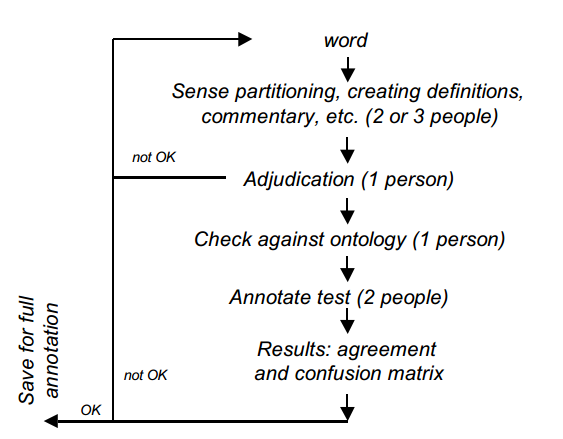
\includegraphics[scale = 0.6]{ontonotes.png}
\caption{OntoNotes Annotation Procedure \citep{Hovy:2006}}
\label{fig:ontonotes}
\end{center}
\end{figure}

\section{Feature Engineering}
\label{section:featureEngineering}
In this section, we describe the feature space construction. We derive features from the structure of WordNet and other available lexical resources. Our features can be broadly categorized into two parts: derived from WordNet and derived from other corpora.  WordNet based features are further subdivided into similarity measures and features. 
Many of the listed features are motivated by \citep{snow07mergesense} and \citep{Mihalcea01ez.wordnet:principles}.

\subsection{WordNet based Features}
\subsubsection{Similarity Measures} 
\label{section:similarityMeasures}
\begin{enumerate}
\item \textbf{Wu and Palmer's Conceptual Similarity}: WUP Similarity \citep{WuPalmer:1994} between concepts $a$ and $b$ in a hierarchy, given as
\begin{align}
sim_{WUP}(a,b) = \frac{2 \times depth(lso(a,b))}{len(a,lso(a,b)) + len(b,lso(a,b)) + 2 \times depth(lso(a,b))} \label{eq:WUP}
\end{align}

Here $depth(lso(a,b))$ is the global depth of the lowest super ordinate of $a$ and $b$ and $len(a,b)$ is the length of the path between the two nodes $a$ and $b$ in the hierarchy.

\item \textbf{Leacock and Chodorow's Normalized Path Length}: LCH Similarity \citep{LCH:1998} between concepts $a$ and $b$ in a hierarchy is given by:
\begin{align}
 sim_{LCH}(a,b) = -\log\left(\frac{len(a,b)}{2 \times \underset{c \in WordNet}{\mbox{max}} depth(c)}\right) \label{eq:LCH}
\end{align}

\item \textbf{Resnik's Information Theory Based Approach}: Information Content for a concept $C$ in the taxonomy is defined as $-\log_2p(c)$, where $p(c)$ is the probability of encountering an instance of concept $c$. Resnik's similarity, introduced in \citep{Resnik:1995}, is given by
\begin{align}
sim_{RES}(a,b) = - \log p (lso(a,b)) \label{eq:Resnik}
\end{align}
Observe that in a taxonomy with a unique top node, the similarity between a pair of concepts having the top most node as their most-specific subsumer will be 0.

\item \textbf{Jiang and Conrath's Combined Approach}: JCN distance \citep{JCN:1997} between concepts $a$ and $b$ is given by:
\begin{align}
dist_{JCN}(a,b) &= IC(a) + IC(b) - 2 \times  IC(lso(a,b)) \label{eq:JC1}\\
&= 2 \log p(lso(a,b)) - (\log p(a) + \log p(b)) \label{eq:JC2}
\end{align}

We use the inverse of JCN distance as a feature, which we call JCN similarity.

\item \textbf{Lin's Universal Similarity Measure}: Lin's measure of similarity between two concepts $a$ and $b$ in a hierarchy, proposed in \citep{Lin:1998}, is given by :
\begin{align}
sim_{LIN}(a,b) = \frac{2 \times \log p(lso(a,b))}{\log p(a) + \log p(b)} \label{eq:Lin}
\end{align}

\item \textbf{Lesk Variants}: We use the following variants of Lesk Similarity \citep{Lesk:1986} as features: Adapted Lesk\citep{Banerjee:2002}, Adapted Lesk Tanimoto and Adapted Lesk Tanimoto without hyponyms. The Adapted Lesk Tanimoto is a variant of Adapted Lesk, where we use the glosses of all the directly related senses and the hyponyms of the hypernym of the sense as well. Jaccard-Tanimoto Coefficient is then calculated over two vectors containing the count of each word in the expanded gloss. The Adapted Lesk Tanimoto No Hyponyms is a simpler version of Adapted Lesk Tanimoto in which we only use direct WordNet relations.
\end{enumerate}

We illustrate the similarity values obtained using above measures in table \ref{tab:similarityMeasuresIllustration} on the following pairs of synsets: 
\begin{itemize}
\item \{\textit{student\#n\#1, pupil\#n\#1, educatee\#n\#1}: a learner who is enrolled in an educational institution\} and \{\textit{student\#n\#2, scholarly\_person\#n\#1, scholar\#n\#1, bookman\#n\#1} : a learned person (especially in the humanities); someone who by long study has gained mastery in one or more disciplines\}
\item \{\textit{student\#n\#1, pupil\#n\#1, educatee\#n\#1}: a learner who is enrolled in an educational institution\} and \{\textit{teacher\#n\#1, instructor\#n\#1} : a person whose occupation is teaching \}
\end{itemize}

\begin{center}
\begin{longtable}{| c | c | c |}  
\hline
\textbf{Similarity Measure} & \textbf{Pair 1} & \textbf{Pair 2} \\ \hline
LCH & 2.0794 & 1.7429 \\ \hline
WUP & 0.8 & 0.7272 \\ \hline
JCN & 0.0984 & 0.0905  \\ \hline
LIN & 0.2725 & 0.2562 \\ \hline
RES & 1.9033 & 1.9033 \\ \hline
AdapLesk & 530.0 & 170.0 \\ \hline
AdapLeskTani & 0.1459 & 0.0696 \\ \hline
AdapLeskTaniNoHypo & 0.1742 & 0.1471 \\ \hline
\caption{Similarity Measures Illustration}
\label{tab:similarityMeasuresIllustration}
\end{longtable}
\end{center}

\begin{comment}
1: 0 2.0794415416798357
1: 1 0.8
1: 2 0.0984253784312118
1: 3 0.27255086834319175
1: 4 1.9033026456664381
1: 5 530.0
1: 6 0.14593596059113303
1: 7 0.17427385892116182
------------------------------
1: 0 1.742969305058623
1: 1 0.7272727272727273
1: 2 0.09047925594509129
1: 3 0.2561841672684562
1: 4 1.9033026456664381
1: 5 170.0
1: 6 0.06958762886597938
1: 7 0.14709677419354839
\end{comment}

\subsubsection{Features}
\begin{enumerate}
%\item Common antonym synsets count \cite{Mihalcea01ez.wordnet:principles} % not applicable for nouns -- not implemented
\item \textbf{Common word lemmas count}: Number of lemmas common in two synsets
\item \textbf{SenseCount}: maximum polysemy degree among the lemmas shared by the synsets
\begin{equation*}
\underset{lemma \in Synset_1 \cap Synset_2}{\max} \mbox{Number of Senses}(lemma)
\end{equation*}

\item \textbf{SenseNum}: number of lemmas having maximum polysemy degree among the lemmas shared by the synsets
\begin{equation*}
\left|\underset{lemma \in Synset_1 \cap Synset_2}{\arg\max} \mbox{Number of Senses}(lemma)\right|
\end{equation*}

\item \textbf{Same lexicographer file}: Synsets in WordNet are divided in several broad categories by the lexicographers. For more details visit Appendix \ref{appendix:lexicographerFiles}.
We check whether two synsets have the same category or not. 

%\item Common verb frames count
%\item Common verb group \cite{Mihalcea01ez.wordnet:principles}

\item \textbf{SP1\_1 merge heuristic} \citep{Mihalcea01ez.wordnet:principles}: Binary feature which is set if S1 and S2 are two synsets containing at least 2 words, and if S1 and S2 contain the same words.
\item \textbf{SP1\_2 merge heuristics} \citep{Mihalcea01ez.wordnet:principles}: Binary feature which is set if S1 and S2 are two synsets with the same hypernym and contain the same words. The strict heuristic checks whether all the hypernyms are shared or not whereas the relaxed heuristic checks if the synsets have at least 1 common hypernym.
\item \textbf{SP1\_3 merge heuristic} \citep{Mihalcea01ez.wordnet:principles}: Binary feature which is set if S1 and S2 are two synsets with at least $K$ words in common. We set $K=3$ here, which makes it equivalent to the \textit{twin relation}.

\item \textbf{Number of common hypernyms}: the number of common hypernyms between the two synsets.

\item \textbf{Autohyponymy}: Whether the two synsets have a hyponym-hypernym relation between them.

\end{enumerate}

\subsection{Features derived from other Corpora}
\subsubsection{eXtended WordNet Domains} eXtended WordNet Domains Project \citep{Gonzalez:XWND} provides us the score of a synset with respect to a domain-label. The dataset contains 169 labels(excluding factotum label) which are hierarchically organized for different POS. We obtain a representation of a synset in the domain label space and use cosine similarity, L1 Distance and L2 Distance computed over the weight representations of the synsets as features.

\subsubsection{BabelNet} BabelNet \citep{NavigliPonzetto:12aij} provides us with two very important datasets of usage. 
One of them is the translation of noun word senses in 6 languages namely: English, German, Spanish, Catalan, Italian and French. Secondly mapping of noun synsets to  \href{http://dbpedia.org/About}{DBpedia} entries. 
For features we use counts of common lemmas in all 6 languages and count of common dbPedia entries.

The idea to cluster word senses using translation equivalences was proposed first in \citep{Resnik:1999:TranslationEquivalences}.

\subsubsection{SentiWordNet} SentiWordNet \citep{Baccianella10sentiwordnet3.0} provides us with a mapping from a synset to a triad of three weights. The weights correspond to the score given to a synset based on its objectivity and subjectivity(positive and negative). For eg.
\begin{itemize}
\item The synset \{\textit{sprightliness\#n\#1, spirit\#n\#7,  liveliness\#n\#2,  life\#n\#9}: animation and energy in action or expression; ``it was a heavy play and the actors tried in vain to give life to it`` \} has the score (P: 0.25, O: 0.75, N:0)
\end{itemize}

We use cosine similarity, L1 Distance and L2 Distance of the weight representations of the synsets as features.

\subsubsection{Mapping of WordNet to Oxford English Dictionary(OED)} 
We derive one of our feature from the sense clusterings produced by mapping WordNet senses to OED senses using Structural Semantic Interconnections method \citep{Navigli05SSI} by organizers of coarse-grained AW task in SemEval-2007\footnote{\url{http://lcl.uniroma1.it/coarse-grained-aw/}} \citep{navigli-litkowski:SemEval-2007}. For each pair of synsets, we check if there are senses in the synsets such they belong to same cluster in the OED mapping.

\section{Classifier and Training}
\label{sec:ClassifierAndTraining}
We train Support Vector Machines using features described in section \ref{section:featureEngineering} on the dataset of synset pairs mentioned in section \ref{section:goldStandardDatasets}, in which every synset pair is given either a ``merged'' or ``not-merged'' label. We will now discuss Support Vector Machines and various normalization techniques and kernels, for completeness.

\subsection{Support Vector Machines}
Support Vector Machines, proposed by \citep{vapnikSVM:95}, are linear machines which try to separate instances of opposite classes by constructing an optimal hyperplane having the largest possible margin. They are widely used for classification tasks and are known for their high accuracies and robustness. An example of such hyperplane is illustrated in figure \ref{fig:svm}. 

\begin{figure}[h]
\begin{center}
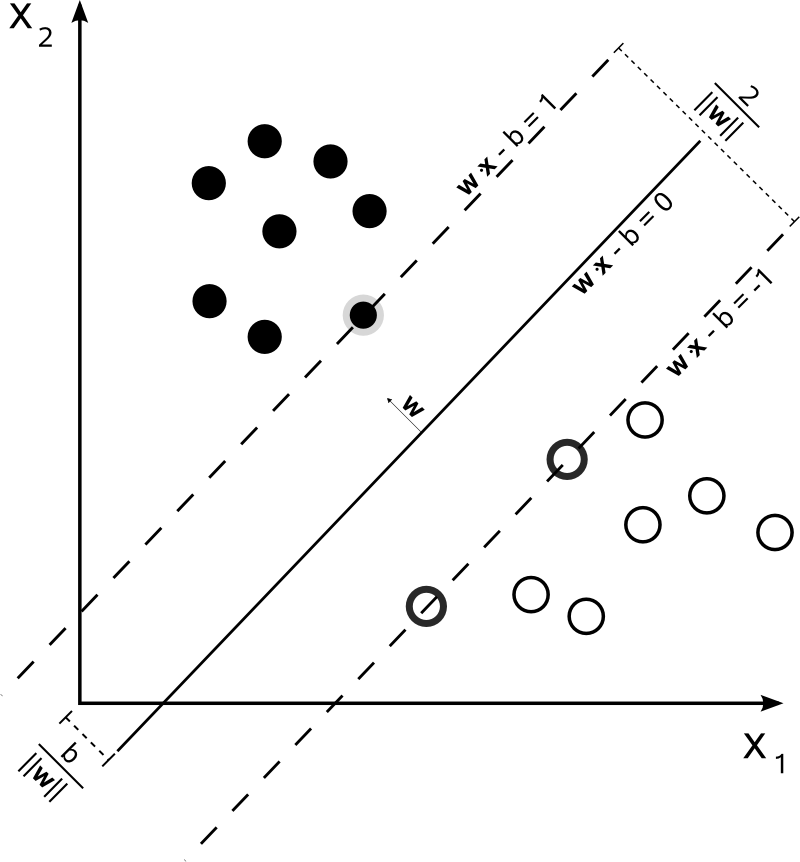
\includegraphics[scale = 0.3]{Svm_max_sep_hyperplane_with_margin.png}
\caption{SVM with maximum margin hyperplane (Source: Wikipedia)}
\label{fig:svm}
\end{center}
\end{figure}

In many applications, non-linear classifiers provide better accuracies than linear classifiers as they are able to discover better decision boundaries. But linear classifiers have advantages over non-linear classifiers as they often have simple training algorithms that scale well with the number of examples. \citep{VapnikSVMKernel:92} introduced the idea of kernels which use the machinery of linear classifiers to discover non-linear decision boundaries by fitting the maximum-margin hyperplane in a transformed feature space. Some common kernels include:
\begin{itemize}
\item Polynomial: $k(\bm{x_i},\bm{x_j}) = (\bm{x_i \cdot x_j})^d$
\item Gaussian Radial Basis Function: $k(\bm{x_i},\bm{x_j}) = exp(-\gamma||\bm{x_i - x_j}||^2)$
\end{itemize}
We experiment with the standard linear kernel and the RBF kernel.

\subsection{Feature Normalization}
Feature Normalization plays a very important role in many learning and optimization algorithms. In practice, many methods work best after the data has been normalized and whitened. Since Support Vector Machine algorithms are sensitive to scaling and have been shown to give better results with normalization, we experiment with two ideas - feature scaling and feature standardization:

\subsubsection{Feature Scaling}
One of the simplest methods to normalize features is to scale the ranges of features to a common range, [-1,1] in our case. The main advantage offered by scaling is that it avoids attributes in smaller numeric ranges being dominated by attributes in greater numeric ranges. It also avoids numerical difficulties like overflow errors caused by large attribute values. Note that both training and testing data should be scaled with the same parameters, otherwise the results would be erroneous. The transformation is obtained by:
\begin{equation}
\label{eq:FeatureScaling}
x' = minReqd + (maxReqd-minReqd)*\left(\frac{x-min}{max-min}\right)
\end{equation}

\subsubsection{Feature Standardization}
For a heterogeneous feature space, feature standardization makes the values of each feature in the data have zero-mean and unit-variance. The following transformation formula achieves the zero-mean and unit-variance requirements:
\begin{equation}
\label{eq:FeatureStandardization}
x' = \frac{x-\mu}{\sigma}
\end{equation}

The mean($\mu$) and variance($\sigma^2$) used in equation \ref{eq:FeatureStandardization} are the sample mean and unbiased sample variance, estimated from the training data. Note that the same transformation must be applied to train and test data to obtain meaningful results.

\section{Implementation}
In this section, we outline some of the important resources which have been used in the implementation: 
\begin{itemize}
\item Access to the WordNet graph was facilitated by extJWNL \footnote{\url{http://extjwnl.sourceforge.net/}}.

\item For WordNet based Word Similarity, we make use of Java WordNet::Similarity \footnote{\url{http://www.sussex.ac.uk/Users/drh21/}} by David Hope, which is a pure Java implementation of Ted Pedersen's Perl WordNet::Similarity \footnote{\url{http://wn-similarity.sourceforge.net/}}.

\item The BabelNet based features were obtained using the BabelNet API \citep{NavigliPonzetto:2012acl}.

\item To train the support vector machine classifier we used SVM implementation by \citep{Joachims98makinglarge-scale}, whose java access is provided by JNI-SVMLight \footnote{JNI-SVMLight: \url{http://adrem.ua.ac.be/~tmartin/}} library.

\item For Information Gain and Gain Ratio study in section \ref{section:InformationGainAndGainRatioStudy}, we use Weka software \citep{wekaSoftware}.
\end{itemize}

\section{Experimental Setup and Evaluation}
\label{section:SupervisedExperimentalSetupAndEvaluation}
\subsection{Train and Test datasets}
Since the quality assurance of Ontonotes dataset is reasonably high and no information is available about Senseval-2 dataset, we use binary classification dataset obtained from OntoNotes for training and validation. We split our dataset into a training set(70\%) and a held-out validation set(30\%). 
\begin{center}
\begin{longtable}{| l | l |}      
    \hline
    Examples & Nouns \\ \hline    
    Positive Examples\footnote{Pair of synsets merged by annotators} & 1214 \\ \hline
    Negative Examples\footnote{Pair of synsets not merged by annotators} & 11974 \\ \hline
    Percentage of Positive examples & 9.20 \\ \hline
    Positive Training examples in random 70\% sample & 850 \\ \hline
    Negative Training examples in random 70\% sample & 8382 \\ \hline
    Positive Testing examples in random 30\% sample & 364 \\ \hline
    Negative Testing examples in random 30\% sample & 3612 \\ \hline    
    \caption{Statistics of Pairwise Classification Dataset}
  \label{tab:pairwiseData}
\end{longtable}
\end{center}
\begin{comment}
\begin{center}
\begin{longtable}{| l | l | l |}      
    \hline
    Examples & Nouns & Verbs \\ \hline    
    Positive Examples\footnote{Pair of synsets merged by annotators} & 1214 & 6881 \\ \hline
    Negative Examples\footnote{Pair of synsets not merged by annotators} & 11974 & 20899 \\ \hline
    Percentage of Positive examples & 9.20 & 24.76 \\ \hline
    Positive Training examples in random 70\% sample & 850 & 4817\\ \hline
    Negative Training examples in random 70\% sample & 8382 & 14630\\ \hline
    Positive Testing examples in random 30\% sample & 364 & 2064\\ \hline
    Negative Testing examples in random 30\% sample & 3612 & 6269\\ \hline    
    \caption{Statistics of Pairwise Classification Dataset}
  \label{tab:pairwiseDataNounVerb}
\end{longtable}
\end{center}
\end{comment}

\subsection{Effect of class distribution in learning}
We trained two systems, which differ in number of negative examples used in training. One uses the whole 70\% dataset extracted and other selects random instances from negative examples of this dataset to get a balanced dataset (equal number of positive and negative instances). For testing, we again used a balanced dataset consisting of equal number of positive and negative instances, disjoint from the training dataset. The former classified all the instances into negative class. We attribute this to the skewed class distribution in the training data. On the other hand, we observe that system 2 learns better boundaries due to the balanced nature of the training set.

Owing to the above observations, for training as well as testing, we used randomly generated balanced datasets(equal number of positive and negative instances - 850 instances from each class) and repeated the process multiple number of times.

\subsection{Effect of normalization schemes and kernels}
\label{section:SVMNormalizationKernelExperiment}
It is known that large margin classifiers are sensitive towards feature scaling and standardization \citep{chang2011libsvm}. To study the same, we experiment with Attribute Normalization techniques and Kernel selection: Min-Max normalization and Z-Score normalization along with Linear and RBF Kernel. 

We perform 5-fold validation i.e. we train the SVM on 5 randomly generated balanced datasets and test them again on a randomly balanced dataset disjoint from the training set. The table \ref{tab:nounExp2} documents the average results of the 5 runs. We report only FScore over both the classes as a measure of performance of the systems. For detailed results of the experiments, refer Appendix \ref{appendix:SVMResults}.

\begin{center}
\begin{longtable}{| c | c | c | c |}      
\hline
Kernel & No Normalization & MinMaxNormalization & ZScoreNormalization\\ \hline
Linear & (0.31, 0.68) & (\textbf{0.73, 0.72}) & (0.05, 0.67)\\ \hline
RBF    & (0.70, 0.37) & (\textbf{0.73}, 0.70) & (0.64, \textbf{0.72})\\ \hline    
\caption{Studying Performance by varying Normalization Schemes and Kernels}
\label{tab:nounExp2}
\end{longtable}
\end{center}

For comparison purposes, we report the performance of the SVM systems, learnt for the 5-fold validation study (described above), on the Senseval-2 Dataset as the test set, in table \ref{tab:nounExp3}.

\begin{center}
\begin{longtable}{| c | c | c | c |}      
\hline
Kernel & No Normalization & MinMaxNormalization & ZScoreNormalization\\ \hline
Linear & (0.15, \textbf{0.90}) & (\textbf{0.44}, 0.81) & (0.01, \textbf{0.90})\\ \hline
RBF    & (0.37, 0.46) & (0.40, 0.69) & (0.41, 0.85)\\ \hline
\caption{SVM Performance on Senseval-2 Dataset}
\label{tab:nounExp3}
\end{longtable}
\end{center}

Observe that both feature normalization as well as kernel selection have a great influence on the classification performance. \citep{chang2011libsvm} report that if the data is not normalized the accuracy of an SVM can severely degrade. Therefore it is important to select the appropriate normalization and kernel for the task.   

For most of the normalization-kernel combinations, the performance is biased towards a particular class. Among the normalization techniques, MinMax Normalization seems to give consistently good performance in both the kernels. So for further studies, we decided to use MinMax Normalization on features. 

Linear Kernel gives better results on both the Senseval-2 dataset and the cross validation, and hence we choose linear kernel over RBF kernel.

\begin{comment}
For MinMax Normalization, the performance difference between linear and RBF kernel is not much. We select Linear kernel for further purposes as it is simpler (Occam's razor) ????
\end{comment}

\subsection{Feature Analysis}
We analyze our feature space in two ways. We evaluate Information Gain and Gain Ratio functions over the features and do a feature ablation study. The former tries to capture the discrimination ability of the feature by itself and the latter tries to measure how a feature corroborates with other features in the feature space.

\subsubsection{Information Gain and Gain Ratio Study}
\label{section:InformationGainAndGainRatioStudy}
\paragraph{Information Gain}
The Information Gain function is based on the notion of entropy, which characterizes the impurity of an arbitrary set of examples distributed among some classes. If an example is randomly selected from a set and its class $c_i$ is announced, then the probability of this announcement is equal to $p_i = \frac{|c_i|}{|D|}$ , and the amount of information it conveys is $-\log_2(p_i)$. The expected information provided by a announcement with respect to the class membership in a dataset $D$, having $m$ classes with estimated class probabilities $p_1,\ldots,p_m$, is given by:
\begin{equation}
Info(D) = -\sum_{i=1}^{m} p_i \log_2(p_i)
\end{equation}

The quantity $Info(D)$ measures the average amount of information(in bits) needed to identify the class of an example in $D$. We consider a similar measurement after $D$ has been partitioned on attribute $A$ in $v$ parts, labeled as $D_1,\ldots D_v$. The amount of information needed to arrive at an exact classification after partitioning using that attribute is the weighted sum over subsets and is given by:

\begin{equation}
Info_A(D) = \sum_{j=1}^v \frac{|D_j|}{|D|} \times Info(D_j)
\end{equation}

The Information Gain is the expected reduction of information requirements caused by knowing the value of $A$ and is given by:
\begin{equation}
Gain_A(D) = Info(D) - Info_A(D)
\end{equation}

\paragraph{Gain Ratio}
The Information Gain function is biased towards tests with many outcomes. To counter the same, Gain Ratio modifies the Information Gain by taking into account the number and sizes of the partitions obtained in a test.

The \textit{split information value} measures the potential information generated by dividing the dataset $D$ into $v$ bins, corresponding to $v$ outcomes on attribute $A$.

\begin{equation}
SplitInfo_A(D) = -\sum_{j=1}^{v}\frac{|D_j|}{|D|} \times \log_2\left(\frac{|D_j|}{|D|}\right)
\end{equation}

The gain ratio is defined as:

\begin{equation}
GainRatio_A(D) = \frac{Gain_A(D)}{SplitInfo_A(D)}
\end{equation}

\paragraph{Evaluation}
We computed all the features over the complete OntoNotes dataset without any normalization and evaluated the same using Information Gain and Gain Ratio as measures. Table \ref{tab:FeatureWiseEvaluation} compares the value for all the features. We highlight the top 7 features according to both the attribute evaluators.

\begin{center}
\begin{longtable}{| c | c | c |}      
\hline
\textbf{Feature} & \textbf{Gain Ratio} & \textbf{Information Gain} \\ \hline
LCH & 0.01288 & \textbf{0.0323} \\ \hline
WUP & 0.0148 & \textbf{0.02899} \\ \hline
JCN & \textbf{0.0215} & 0.02094 \\ \hline
LIN & 0.01943 & 0.02072 \\ \hline
RES & 0.01379 & 0.02335 \\ \hline
AdapLesk & 0.01688 & \textbf{0.03456} \\ \hline
AdapLeskTani & \textbf{0.02306} & \textbf{0.03603} \\ \hline
AdapLeskTaniNoHypo & 0.01685 & \textbf{0.03014} \\ \hline
\hline
Common Lemma Count & 0.00438 & 0.00394 \\ \hline
SenseCount & 0.00293 & 0.00293 \\ \hline
SenseNum & 0.0 & 0.0 \\ \hline
lexFileSimilarity & 0.01552 & 0.01143 \\ \hline
mergeSP1\_1 & 0.00282 & 0.00151 \\ \hline
mergeSP1\_2 & \textbf{0.04195} & 0.00103 \\ \hline
mergeSP1\_2\_relaxed & \textbf{0.04709} & 0.00119 \\ \hline
mergeSP1\_3 & 0.0 & 0.0 \\ \hline
number of Common Hypernyms & \textbf{0.08833} & 0.00965 \\ \hline
autohyponymy & 0.0 & 0.0 \\ \hline
\hline
Domain-Cosine Similarity & \textbf{0.01997} & \textbf{0.04416} \\ \hline
Domain-l1 Distance & 0.00445 & 0.00219 \\ \hline
Domain-l2 Distance & 0.00771 & 0.00238 \\ \hline
OEDMerged & \textbf{0.0326} & \textbf{0.03123} \\ \hline
SentiWordNet-CosineSimilarity & 0.0 & 0.0 \\ \hline
SentiWordNet-l1 Distance & 0.0 & 0.0 \\ \hline
SentiWordNet-l2 Distance & 0.0 & 0.0  \\ \hline
CommonEnglishTranslations & 0.00829 & 0.00671 \\ \hline
CommonGermanTranslations & 0.00732 & 0.00559 \\ \hline
CommonSpanishTranslations & 0.00547 & 0.00445 \\ \hline
CommonItalianTranslations & 0.00505 & 0.00418 \\ \hline
CommonFrenchTranslations & 0.00737 & 0.00634 \\ \hline
CommonCatalanTranslations & 0. 0.00657 & 0.00533 \\ \hline
CommonDBpediaEntries & 0.0 & 0.0 \\ \hline
\caption{Information Gain and Gain Ratio Based Evaluation}
\label{tab:FeatureWiseEvaluation}
\end{longtable}
\end{center}

\subsubsection{Feature Ablation Study}
We divide our features in 6 categories: WordNet Similarity measures, WordNet based features, eXtended WordNet Domains features, BabelNet features, SentiWordNet features and Navigli OED Mappings. 

We report the average F-Score of both the classes observed by removing that category of features from our feature space, retraining and retesting the classifiers on randomly generated balanced datasets, keeping everything else the same. The SVMs are trained using linear kernel and features are normalized using MinMax Normalization for all the experiments reported in this study. The table \ref{tab:nounEvalFeatureAblation} summarises the study.

\begin{center}
\begin{longtable}{| c | c | c |}  
\hline
\textbf{Features Removed} & \textbf{FScore Positive} & \textbf{FScore Negative} \\ \hline
WordNet Similarity Measures & 0.6948 & 0.6784 \\ \hline
WordNet Based Features & 0.7227 & 0.7092 \\ \hline
BabelNet Features & 0.7232 & 0.7127 \\ \hline
Domain Similarity Features & 0.6814 & 0.6619 \\ \hline
OED Feature & 0.6957 & 0.7212 \\ \hline
SentiWordNet Features & 0.7262 & 0.7192 \\ \hline
\hline
\textbf{Without Removing Features} & 0.7262 & 0.7192 \\ \hline
\caption{Feature Ablation Study}
\label{tab:nounEvalFeatureAblation}
\end{longtable}
\end{center}

\subsubsection{Observations}

\paragraph{WordNet Similarity Features}: 
The similarity measures have a significant effect on the performance of the SVMs as can be observed from table \ref{tab:nounEvalFeatureAblation}. This highlights the importance of the underlying ontology structure of the WordNet which these similarity measures try to capture.

Note from table \ref{tab:FeatureWiseEvaluation} that the gloss based features(the lesk variants - refer section \ref{section:similarityMeasures}) have high Information Gain values. This can be attributed to the fact that the annotators primarily rely on gloss descriptions to interpret synsets. In the relatedness study by \citep{mccarthy2006relating}, the annotators only had glosses as evidence to decide if senses were ``related'' or not.

\paragraph{WordNet Based Features}:
Among the WordNet based features, the features relating the synsets to their hypernyms like the ``SP1\_2 merge heuristics'', the number of common hypernyms etc. seem to be discriminatory. This is understandable as the hypernym related feaures capture the notion of semantic generalization, which is essential to undestand a sense. 

\paragraph{BabelNet Features}:
The objective of using multilingual features was to test whether the translation equivalences are powerful enough to capture semantic associations between two word senses. Low values of the Information Gain and Gain Ratio of the BabelNet features reflect that the above heuristic is a weak indicator for sense-merging. 

Using mapping to DBPedia entries as a feature was an effort to harness the DBpedia Knowledge Base \footnote{\url{http://dbpedia.org/About}}. But we observe from table \ref{tab:FeatureWiseEvaluation} that the feature is not that useful. A better use of the DBpedia ontology would be to estimate the similarity of mapped concepts using the underlying hierarchy.

\paragraph{Domain Similarity Features}:
Intuitively, as an annotator, approximately matching the domain of two senses serves as a strong cue about whether the two senses are semantically related enough to be merged. This is justified by the high info-gain and gain-ratio values for the domain similarity features.

\paragraph{Oxford English Dictionary Mapping}:
\citep{Navigli06meaningfulclustering} have already shown the effectiveness of this mapping in a WSD task based setting. High values of Information Gain and Gain Ratio support the same. The problem we face with the feature is its incompleteness as not all the word senses are clustered by mapping to Oxford English Dictionary.

\paragraph{SentiWordNet Features}: 
Another interesting set of features is the SentiWordNet based features. Their removal doesn't affect the system's performance which can be attibuted to the fact that most of the noun synsets in the SentiWordNet project are described as objective concepts. Their non-discriminatory nature is substantiated by the Information Gain and Gain Ratio based study as well (refer table \ref{tab:FeatureWiseEvaluation}). 

\section{Discussion}
In this section, we would like to address some concerns regarding the similarity function learnt.

\subsection{Inconsistent Predictions} 
\label{section:SVMInconsistentPredictions}
Using the outputs of the SVM learnt directly as the similarity distance poses the problem of inconsistent predictions i.e. it can happen that for three synsets $A$, $B$ and $C$, $sim_{SVM}(A,B) > 0$ and $sim_{SVM}(B,C) > 0$ while $sim_{SVM}(A,C) < 0$. Such inconsistencies, though rare, can happen. Even the human annotators involved in preparation of Senseval-2 dataset \citep{Senseval2LexicalSampleTask} have made such errors. This motivates us to utilize the WordNet structure to correct such inconsistencies. % I can give exact number here !

\subsection{Coverage of the SVM} 
The training data for the SVM is not representative of the WordNet synsets because we trained only on the synset pairs that have atleast one lemma in common. It is interesting to note here that the number of synsets which contain atleast one polysemous lemma is only 33155 out of total 82115 synsets. This questions the idea of using the SVM models learnt as generic synset similarity estimators. 

\citep{snow07mergesense} addresses this issue by taking similarity between synsets not sharing any word as $0$ and for the synsets sharing atleast a word as the prediction by the SVM, for the purpose of sense-merging. Because of the heterogeneous nature of the similarity defined by \citep{snow07mergesense}, it does not serve as a generic synset similarity measure.

\subsection{Insufficient Data for Learning}
The SVMs were learnt on randomly selected balanced datasets of 1700 instances with 850 instances of each class. Though the results are promising, the number of training instances is small as compared to the total number of synsets involved (33155), which makes it tough to judge whether the similarity metric learnt is generic enough or not.

\section{Conclusions and Future Work}
\citep{mccarthy2006relating} performed an annotation study in which 3 native english speakers were asked to label around 300 sense pairs as ``related'', ``unrelated'' or ``don't know''. The inter-annotator F-Scores were (0.7926, 0.5454, 0.4874)\footnote{Since the annotation was done by native speakers and not experienced linguists or lexicographers, we can expect a slightly higher inter-annotator F-Score for the task.} \citep{mccarthy2006relating} \citep{snow07mergesense}. These figures highlight that humans differ in their tendency to split or lump senses and that the task is inherently a difficult one.

Significant advancement of supervised learning algorithms over the last two decades and their ability to capture the relative importance of features essential to the task in hand inspired us to utilize their potential in understanding the importance of the various features in merging synsets.

The use of external corpora for supervision is motivated by the fact that we are not able to fully capture the information in WordNet for e.g. we are not able to utilize the gloss of the synset beyond lexical measures. By enriching the semantic information of the synsets using features like belongingness to different domains, sentiment associated with them etc. we are able to improve the performance of our systems. 

The evaluation suggests that there is a need to enrich WordNet along with the production of additional resources to better understand word senses. Some such efforts include augmenting WordNet with teleological links \footnote{\url{http://wordnetcode.princeton.edu/standoff-files/teleological-links.xls}}, morphological and semantic information \citep{morphosemanticLinks}. 